\documentclass{article}

\usepackage{graphicx} % more modern
\usepackage{subfigure} 
\usepackage{amssymb}
\usepackage{amsmath}
\usepackage{amsthm}
\usepackage{epstopdf} 

% For citations
\usepackage{natbib}

% For algorithms
\usepackage{comment}
\usepackage{framed}
\usepackage{algorithm}
\usepackage{algorithmic}
\usepackage{amsmath}
%\usepackage{algorithmicx}
%\usepackage{algpseudocode}

\usepackage{hyperref}

\allowdisplaybreaks

\newcommand{\theHalgorithm}{\arabic{algorithm}}

\newtheorem{theorem}{Theorem}[section]
\newtheorem{lemma}[theorem]{Lemma}
\newtheorem{conjecture}[theorem]{Conjecture}
\newtheorem{proposition}[theorem]{Proposition}
\newtheorem{definition}[theorem]{Definition}
\newtheorem{corollary}[theorem]{Corollary}

\usepackage[accepted]{icml2014}  % XXX : just set temporarly to print out authors corretly.
%\usepackage{icml2014}  

\renewcommand{\algorithmicrequire}{\textbf{Input:}}
\renewcommand{\algorithmicensure}{\textbf{Output:}}

\begin{document} 

\icmltitle{Understanding structure of parameters in neural networks}

\icmlauthor{Emily Denton}{denton@cs.nyu.edu}
\icmlauthor{Wojciech Zaremba}{zaremba@cs.nyu.edu}
\icmlauthor{Joan Bruna}{bruna@cs.nyu.edu}
\icmlauthor{Rob Fergus}{fergus@cs.nyu.edu}

\icmlkeywords{machine learning, deep learning, low-dimensional structure, redundancies in neural networks}

\begin{abstract}

\end{abstract}

\section{Introduction}
Main criticism of neural networks is in the lack of interpretability of their results. This is serious issue,
as it hinders process of knowledge injection, and makes difficult to predict their behaviour in the new conditions (not
presented during training). This issue is the consequence of superficial understanding of computation 
underlaying neural networks. We do attempt in direction of understanding computation behind neural networks.


We show that learnt parameters of neural networks have very
rich low-dimensional linear structure. We are not able to explain reason for its presents. However, 
such a structure has a far-reach consequences in (i) understanding computation of neural networks, 
(ii) regularization of neural networks, (iii) optimization, (iv) accelerating testing, (v) re-parametrization.
We describe how such structure can be extracted and visualized. We show it for state-of-the-art object recognition models ($\sim60$ mln. 
learnable parameters). Moreover, we explore consequences of this low-rank linear structure for simpler models. 


\section{Related Work}


Our low-rank approximations get inspired by work of \cite{denil2013predicting} on redundancies in neural 
networks. They shown that based on small fraction of weights (e.g. $\sim 5\%$), one can accurately 
predict rest of weights. This indicates that neural networks are heavily over-parametrized.
All the methods presented here focus on exploiting linear structure of such over-parametrization.


\section{Low Rank Approximations}
In this section, we give theoretical background on low-rank approximations. First, we discuss simplest setting, which is
for matrices (two dimensional tensors). Further, we move to approximation of 4-dimensional tensors with 2 convolutional (spacial)
dimensions.


\subsection{Matrix Low Rank Approximation}
Let's consider input $X \in \mathbb{R}^{n \times m}$, and matrix of weights $W \in \mathbb{R}^{m \times k}$.
$W$ might have a low-rank (many eigenvalues close to zero), and matrix multiplication of $X$ with $W$ might be 
very close to the matrix multiplication with approximation of $W$. 


Every matrix can be expressed using singular value decomposition:
\begin{equation*}
	W = USV^T\text{, where }U \in \mathbb{R}^{m \times m}, S \in \mathbb{R}^{m \times k}, V \in \mathbb{R}^{k \times k}
\end{equation*}
$S$ is has eigenvalues on the diagonal, and apart from it has zeros. $W$ can be approximated by using $t$ most significant
eigenvalues from $S$. We can write approximation as
\begin{equation*}
	\hat{W} = \hat{U}\hat{S}\hat{V}^T\text{, where }\hat{U} \in \mathbb{R}^{m \times t}, \hat{S} \in \mathbb{R}^{t \times t}, \hat{V} \in \mathbb{R}^{t \times k}
\end{equation*}

\subsection{Tensor Low Rank Approximations}

In typical object recognition architectures, the convolutional tensors resulting
from the training exhibit strong redundancy and regularity across all its 
dimensions. A particularly simple way to exploit such regularity is to 
linearly compress the tensors, which amounts to finding low-rank 
approximations.

Convolution kernels can be described as a $4$-dimensional tensors. Let $W \in \mathbb{R}^{C \times X \times Y \times F}$ 
be convolutional kernel. 
$C$ is input number of feature maps (or colors), $X, Y$ are special dimensions
over which we compute convolution, and $F$ is the target number of feature maps.
Let $I \in \mathbb{R}^{C \times N \times M}$ denote an input signal.
A generic convolutional layer is defined as
\begin{align*}
\label{convlayereq}
&I \ast W (f,x,y) = \\
&\sum_{c=1}^C \sum_{x'=-X/2}^{X/2} \sum_{y'=-Y/2}^{Y/2} I(c,x-x',y-y') W(c,x',y',f)
\end{align*}

Low-rank approximation of tensors is very similar to low-rank approximation of matrices.
However, first we have to choose $2$ dimensions with respect to which we are approximating, and treat
rest of tensor as it would be a matrix. 

\subsubsection{Monochromatic filters}
For generic convolution there are connections between all output feature maps, and all input feature maps.
However, one could imagine that this connections in trained network in some basis could become sparse. 

\section{Consequences}

\subsection{Understanding computation of neural networks}
Low-rank analysis can reveal underlaying computation. Moreover, it can be a corner stone
in understanding why neural networks works. In this section, we treat this topic briefly 
(it is focus of a future work), and we show evaluation for a simple network trained to classify MNIST.


We took networks considered previously during development of dropout \cite{hinton2012improving}.
We look on trained filters from fully-connected layers from perspective of low-rank analysis.
First, we trained fully connected 768-800-800-10 with, and without $50\%$ dropout until convergence.
Figure \ref{filters_mnist} compares arbitrary filters of such networks versus left-singular values. 
Moreover, it can be quantified that left-singular values for dropout network are better than for non dropout network. 


Edges of MNIST dataset are almost empty, and pixels over there have very small discriminative power. 
Classifier, which base its decision on values there is likely to overfit. Robust classifier should
match strokes, rather than small details. We wanted to measure how much
dropout based, and non-dropout based classifier relies on values from edges of images.
We took the same 768-800-800-10 networks, and computed average norm over strips from
the top, bottom, left side, and right side of the filters, and respectively of the left-singular values of filters. 
We took 10 left-singular values, and all the filters. Table \ref{overfit} presents numerical results.

\begin{figure}[h]
\centering
  \subfigure[Visualization of arbitrary filters for fully connected MNIST network.]{
      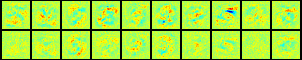
\includegraphics[width=0.95\linewidth]{img/filters_mnist.png}
      \label{filters_no_svd_mnist}
  }\
  
  \subfigure[Visualization of left singular vectors for fully connected MNIST network.]{
      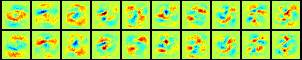
\includegraphics[width=0.95\linewidth]{img/filters_svd_mnist.png}
      \label{filters_svd_mnist}
   }
\caption{Visualization of filters for fully connected network trained on MNIST dataset. For every subfigure, first 
	 row is a network trained with dropout, and the second is trained without.}
\label{filters_mnist}
\end{figure}

\begin{table}
\tiny
\centering
\begin{tabular}{rrr}
\hline
Degree & Grammar size & Time (s) \\
\hline
2 & 5 & 17 \\
3 & 15 & 188 \\
4 & 48 & 2535\\
5 & 139 & 31320 \\
6 & 437 & 434681 \\
\hline
\end{tabular}
\caption{aaaaaaaa}
\label{overfit}
\end{table}


% visualization of principle components for mnist, mnist dropout, vs a single filter.

\subsection{Regularization}

\subsection{Speeding up testing}
Training large neural networks (NN) takes weeks, or even months. This can hinder 
research, and there have been extensive effort devoted to speed up training procedure.
However, resource-wise from perspective of companies executing neural networks on internet-scale
data (e.g. annotating images), this is not the main cost. Major cost is in the 
final stage, where network is evaluated on the target data, which is present in quantities of billions.
We focus here on speeding up evaluation of \emph{trained} NN, which directly
maps to the cost of executing NN on internet-scale data. 


\section{Numerical Experiments}

\subsection{MNIST}

\subsection{Imagenet}

\subsubsection{First layer analysis}

% Run on two imagenets
% Show denoising.
% Show two planes, and axises. Superimpose transparent planes, and axises.
% Project to subspaces and show test error (maybe even run on 50k).
% Present filters mapping to planes.

\begin{figure}[h]
\centering
\mbox{
  \subfigure[aaa]{
      \includegraphics[width=0.55\linewidth]{img/RGB_components_matthew_3d.eps}
      \label{RGB_components_matts_3d}
  }\quad
  \subfigure[aaa]{
      \includegraphics[width=0.55\linewidth]{img/RGB_components_matthew_3d-2.eps}
      \label{RGB_components_matts_3d-2}
   }\quad
}
\caption{Experiment results}
\end{figure}

\begin{figure}[h]
\centering
\mbox{
  \subfigure[aaa]{
      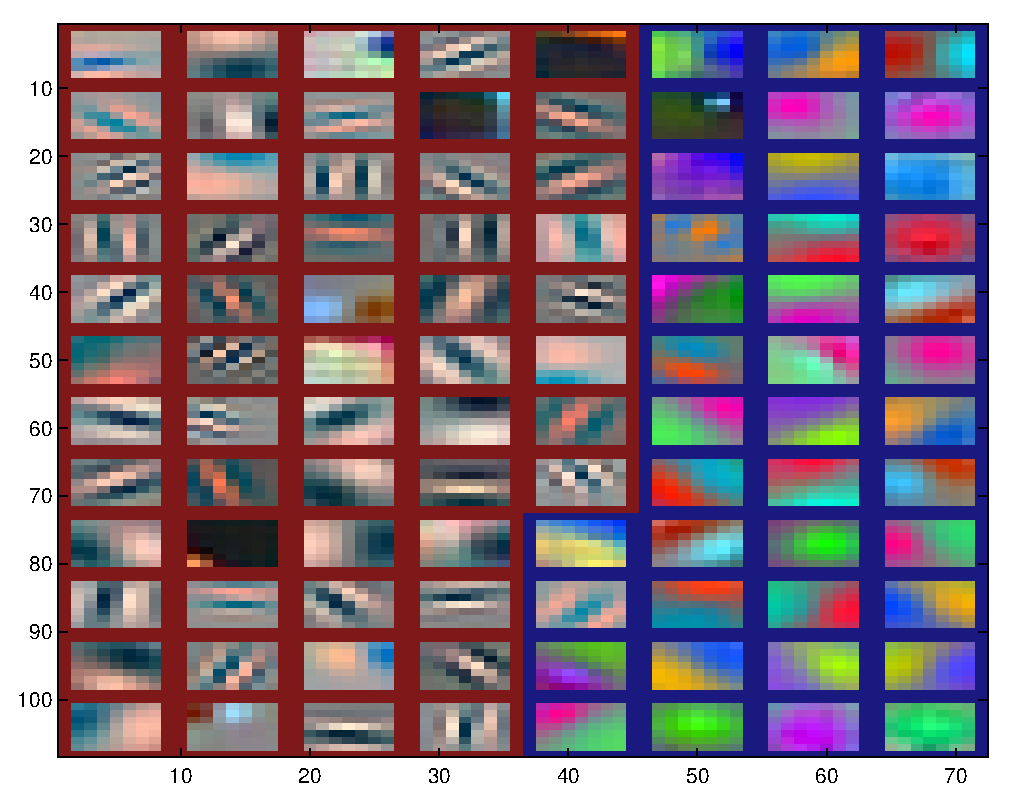
\includegraphics[width=0.55\linewidth]{img/first_layer_filters_clustered_matthew.eps}
      \label{first_layer_filters_clustered_matthew.eps}
  }\quad
}
\caption{First layer filters grouped by subspace cluster}
\end{figure}

\subsubsection{Further layers analysis}


\section{Discussion}

\nocite{*}
\bibliography{bibliography}
\bibliographystyle{icml2014}


\end{document}
